\documentclass{beamer}
% imprimir
% \documentclass[handout]{beamer} 
% \usepackage{pgfpages}
% \pgfpagesuselayout{4 on 1}[a4paper,landscape,border shrink=5mm]

\mode<presentation> {
  \usetheme{Warsaw}
  \setbeamercovered{transparent}
}

\usebackgroundtemplate{
\includegraphics[width=\paperwidth]{format/libresoft-bg.png}}
\usepackage[spanish]{babel}
\usepackage[utf8]{inputenc}

\usepackage{times}
\usepackage[T1]{fontenc}

%% Metadatos del PDF.
\hypersetup{  
  pdftitle={Clusters de ALta Disponibilidad},
  pdfauthor={Miguel Vidal},
  pdfcreator={GSyC/Libresoft},
  pdfproducer=PDFLaTeX,
  pdfsubject={Virtualización con Qemu},
}
%%


\defbeamertemplate*{footline}{shadow theme}
{%
  \leavevmode%
  \hbox{\begin{beamercolorbox}[wd=.5\paperwidth,ht=2.5ex,dp=1.125ex,leftskip=.3cm plus1fil,rightskip=.3cm]{author in head/foot}%
    \usebeamerfont{author in head/foot}\insertframenumber\,/\,\inserttotalframenumber\hfill
\includegraphics[scale=0.40]{format/cc-by-80x15.png} \hspace{0.1cm}\insertshortauthor 
% \usebeamerfont{author in head/foot} 
\includegraphics[width=0.7cm]{format/cc-by.png} \hfill\insertshortauthor
  \end{beamercolorbox}%
  \begin{beamercolorbox}[wd=.5\paperwidth,ht=2.5ex,dp=1.125ex,leftskip=.3cm,rightskip=.3cm plus1fil]{title in head/foot}%
    \usebeamerfont{title in head/foot}\insertshorttitle%
  \end{beamercolorbox}}%
  \vskip0pt%
}

\begin{document}

\title{Clusters de Alta Disponibilidad}
\subtitle{Conceptos básicos}
\author{Miguel Vidal \and José Castro}
\institute{\{mvidal,jfcastro\}@libresoft.es} 
\date[CASUL 2011]{Curso de Arquitectura de Servidores, 2011}

\frame{
\maketitle
\begin{center}

\includegraphics[width=6cm]{format/gsyc-urjc}
\end{center}
}

%% License slide
\begin{frame}
  \vspace{2cm}
  \begin{flushright}
    {\small (cc) 2011 Miguel Vidal, Jose Castro.} \\
%    \vspace{0.25cm}
    \medskip
    {\scriptsize Esta presentación se distribuye bajo \\ licencia Creative Commons Reconocimiento 3.0 España}
%    \vspace{0.10cm}
  \end{flushright}
  \begin{center}
    \href{http://creativecommons.org/licenses/by/3.0/es}{
\includegraphics[width=2cm]{format/cc-by.png}} \\
    {\tiny \url{http://creativecommons.org/licenses/by/3.0/es}}
  \end{center}
\end{frame}%%


\usebackgroundtemplate{}


%%%%%%%%%%%%%%%%%%%%%%%%%%%%%%%%%%%%%%%%%%%%%%%%%%%%%%%%%%%%%%%%%%%%%%%

\begin{frame}
\frametitle{¿Qué es un clúster HA?}


\begin{block}{Cluster}
Conjunto de dos o más máquinas unidas por red.
\end{block}

\begin{block}{Alta Disponibilidad}
24/7, alto grado de fiabilidad y de continuidad operativa.
\end{block}


\begin{definition}
\alert{Cluster HA}: Conjunto de dos o más máquinas orientado a ofrecer y garantizar servicios en \alert{Alta Disponibilidad}. 
\end{definition}

\end{frame}

%%%%%%%%%%%%%%%%%%%%%%%%%%%%%%%%%%%%%%%%%%%%%%%%%%%%%%%%%%%%%%%%%%%%%%%

\begin{frame}
\frametitle{¿Qué es un clúster HA?}

\begin{itemize}

\item Se basa en 2 o más máquinas redundantes (\alert{nodos}), que asumen el servicio cuando algún componente del sistema falla.
\item El software de alta disponibilidad debe ser capaz de arrancar automáticamente los servicios en cualquiera de las otras máquinas del cluster (\alert{failover}).
\item Se busca eliminar los \alert{Puntos Únicos de Fallo} (SPoF), mediante redundancia a todos los niveles, desde el hardware hasta el almacenamiento o las conexiones de red. 
\end{itemize}

\end{frame}


%%%%%%%%%%%%%%%%%%%%%%%%%%%%%%%%%%%%%%%%%%%%%%%%%%%%%%%%%%%%%%%%%%%%%%%

\begin{frame}
\frametitle{¿Qué es un clúster HA?}

\begin{columns}

\column[t]{4cm}

\begin{figure}[h]

\begin{center}
  \centering
  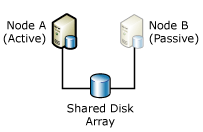
\includegraphics[height=1in]{figs/cluster.png}
%  \caption{Clúster HA de 2 nodos. \textit{Fuente:} Wikipedia.}
\end{center}
\end{figure}


\column[t]{7.5cm}

\begin{itemize}
	\item \alert{Nodos activos} o \alert{maestros}: donde normalmente se ejecuta el servicio.
	\item \alert{Nodos pasivos}, \alert{backups} o \alert{esclavos}: despliegan los servicios en el caso de que el nodo maestro falle. 
\end{itemize}

\end{columns}


\end{frame}


%%%%%%%%%%%%%%%%%%%%%%%%%%%%%%%%%%%%%%%%%%%%%%%%%%%%%%%%%%%%%%%%%%%%%%%

\begin{frame}
\frametitle{Misión de un clúster HA}

Un clúster HA debe ser capaz de: 

\begin{itemize}
\item detectar cualquier fallo en un nodo (hardware o software)
\item reiniciar los servicios en otro nodo (\alert{failover})
\item mantener el servicio sin intervención de operador alguno
\item garantizar la integridad de los datos del clúster
\item Migrar los servicios de nuevo a la máquina original cuando el nodo se recupera (\alert{failback})
\end{itemize}

\bigskip

\small
Puede incluir otras operaciones previas automatizadas, como montar el sistema de ficheros, asignarse la IP, etc. 

\end{frame}

%%%%%%%%%%%%%%%%%%%%%%%%%%%%%%%%%%%%%%%%%%%%%%%%%%%%%%%%%%%%%%%%%%%%%%%

\begin{frame}
\frametitle{Tipos de configuración}

\begin{itemize}
\item El tamaño más frecuente de un clúster HA es de \alert{2 nodos} (mínimo requerido).
\item Los dos configuraciones más comunes en los clusters de dos nodos son:
	\begin{itemize}
	\item \alert{Clúster activo/pasivo}
	\item \alert{Clúster activo/activo}
	\end{itemize}
\item \alert{N+1}: Un nodo extra que puede asumir las funciones de cualquiera de los nodos que haya fallado.
\end{itemize}

\end{frame}


%%%%%%%%%%%%%%%%%%%%%%%%%%%%%%%%%%%%%%%%%%%%%%%%%%%%%%%%%%%%%%%%%%%%%%%

\begin{frame}
\frametitle{Tipos de clusters HA}

\begin{figure}[h]

\begin{center}
  \centering
  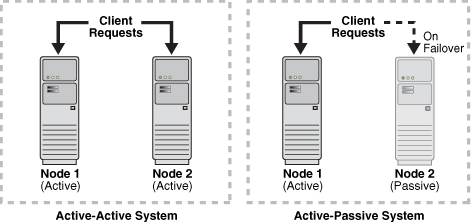
\includegraphics[height=1.7in]{figs/clusters2.png}
%  \caption{Clúster HA de 2 nodos. \textit{Fuente:} Wikipedia.}
\end{center}
\end{figure}

	\begin{itemize}
	\item \alert{Clúster activo/activo}: todos los nodos se encuentran dando servicio.
	\item \alert{Clúster activo/pasivo}: hay un solo nodo dando servicio.
	\end{itemize}

\end{frame}


%%%%%%%%%%%%%%%%%%%%%%%%%%%%%%%%%%%%%%%%%%%%%%%%%%%%%%%%%%%%%%%%%%%%%%%

\begin{frame}
\frametitle{Cluster activo-activo}

\begin{columns}

\column[t]{4cm}

\begin{figure}[h]

\begin{center}
  \centering
  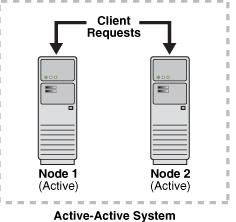
\includegraphics[height=1.7in]{figs/active-cluster.png}
%  \caption{Clúster HA de 2 nodos. \textit{Fuente:} Wikipedia.}
\end{center}
\end{figure}


\column[t]{5cm}
\vspace{2cm}

\alert{Clúster activo/activo}: todos los nodos se encuentran dando servicio.

\end{columns}


\end{frame}


%%%%%%%%%%%%%%%%%%%%%%%%%%%%%%%%%%%%%%%%%%%%%%%%%%%%%%%%%%%%%%%%%%%%%%%

\begin{frame}
\frametitle{Cluster activo-pasivo}

\begin{columns}

\column[t]{4cm}

\begin{figure}[h]

\begin{center}
  \centering
  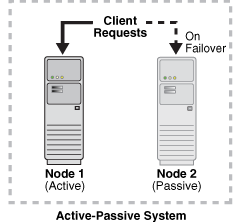
\includegraphics[height=1.7in]{figs/passive-cluster.png}
%  \caption{Clúster HA de 2 nodos. \textit{Fuente:} Wikipedia.}
\end{center}
\end{figure}


\column[t]{5cm}
\vspace{2cm}

\alert{Clúster activo/pasivo}: hay un solo nodo dando servicio.

\end{columns}


\end{frame}


%%%%%%%%%%%%%%%%%%%%%%%%%%%%%%%%%%%%%%%%%%%%%%%%%%%%%%%%%%%%%%%%%%%%%%%

\begin{frame}
% \frametitle{Clúster HA de 2 nodos}

\begin{figure}[h]

\begin{center}
  \centering
  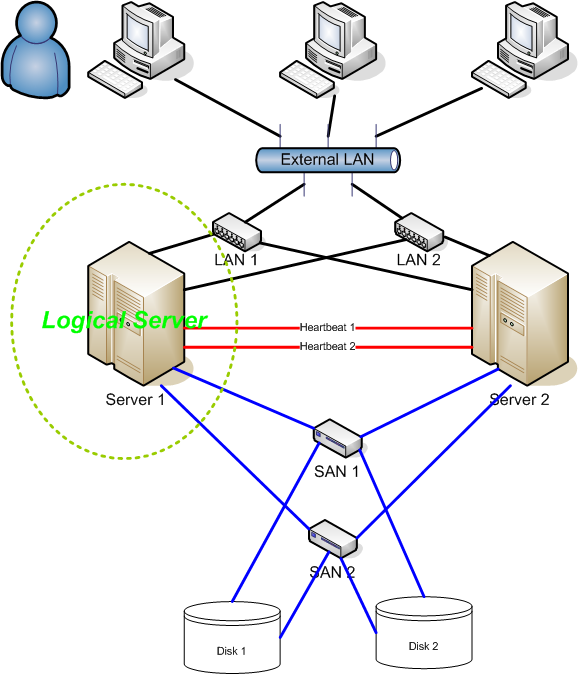
\includegraphics[height=2.7in]{figs/2nodeHAcluster.png}
  \caption{Clúster HA de 2 nodos. \textit{Fuente:} Wikipedia.}
\end{center}
\end{figure}

\end{frame}


%%%%%%%%%%%%%%%%%%%%%%%%%%%%%%%%%%%%%%%%%%%%%%%%%%%%%%%%%%%%%%%%%%%%%%%

\begin{frame}
\frametitle{Conceptos básicos (1)}

\begin{itemize}
\item \alert{Failover}: recuperación de un fallo desplegando los servicios en otro nodo.
\item \alert{Heartbeat}: pulso o ``latido'' mediante el cual se mantiene la comunicación entre los nodos del clúster. 
\item \alert{Split-brain}: cuando los enlaces de red que unen a los nodos entre sí caen, pero los nodos siguen operando. 
\end{itemize}

\end{frame}

%%%%%%%%%%%%%%%%%%%%%%%%%%%%%%%%%%%%%%%%%%%%%%%%%%%%%%%%%%%%%%%%%%%%%%%

\begin{frame}
\frametitle{Conceptos básicos (2)}

\begin{itemize}
\item \alert{Stonith} (``Shoot The Other Node In The Head''): una de las técnicas de \alert{fencing} (bloqueo de recursos en estado incierto). Ambos nodos se ``apuntan'' uno al otro: al detectar que un nodo está caído, el otro nodo le enviará un comando ``reset''. También se usa como técnica de recuperación automática para desbloquear un nodo.
\item \alert{Agente de recurso}: un interfaz estándar para manejar los recursos del cluster (red, montaje de filesystems, servicios, etc.). 
\end{itemize}

\end{frame}


%%%%%%%%%%%%%%%%%%%%%%%%%%%%%%%%%%%%%%%%%%%%%%%%%%%%%%%%%%%%%%%%%%%%%%%

\begin{frame}
\frametitle{Referencias}

\begin{itemize}
\item Linux HA Project: \href{http://www.linux-ha.org}{http://www.linux-ha.org}
\item \textsc{Miguel Vidal, José Castro}: \href{http://www.ati.es/novatica/2011/209/Nv209-75.pdf}{``Creación de un clúster de Alta Disponibilidad''}, \textit{Novática}, nº 209, marzo de 2011. 
\end{itemize}

\end{frame}




%%%%%%%%%%%%%%%%%%%%%%%%%%%%%%%%%%%%%%%%%%%%%%%%%%%%%%%%%%%%%%%%%%%%%%


\frame{
\maketitle
\begin{center}

\includegraphics[width=6cm]{format/gsyc-urjc}
\end{center}
}



\end{document}


